\documentclass[10pt]{article}
\usepackage[margin = 0.75in]{geometry}
\usepackage[doublespacing]{setspace}
\usepackage[hidelinks]{hyperref}
\usepackage[sfdefault]{noto}
\usepackage[T1]{fontenc}
\usepackage[hangul]{kotex} % Korean Version
\usepackage{graphicx, fontawesome, calc, enumitem}
\setlength{\parindent}{0pt}
\setlength{\tabcolsep}{0pt}
\setlist[itemize, 1]{leftmargin = 0.1in}
\setlist[itemize, 2]{leftmargin = 0.3in}
\NewDocumentCommand \TIME { m o } {#1\IfValueTF{#2}{\newline \enspace to #2}{}}
\NewDocumentCommand \HEAD { m } {\raggedleft \textbf{#1} \qquad}

\begin{document}
  \pagestyle{empty}

  \begin{tabular}{ p{.75\linewidth} p{.25\linewidth} }
    % Name
    {\Large 김형준} \newline
    % One-Liner Description
    % Computer Engineer and Software Developer
    서울대학교 전기정보공학부 학사과정 재학 중 \newline
    % Social and Background
    \faLinkedin{} \href{https://www.linkedin.com/in/thekpaul}{@thekpaul} \quad
    \faHome{} \url{https://thekpaul.dev} \quad
    \faFlag{} 대한민국 \newline
    \faGithub{} \href{https://www.github.com/thekpaul}{thekpaul} \quad
    \faInstitution{} \href{mailto:jsvn7777@snu.ac.kr}{jsvn7777@snu.ac.kr} \quad
    \faEnvelopeO{} \href{mailto:thekpaul000@gmail.com}{thekpaul000@gmail.com}
    &
    % Profile Picture
    \multicolumn{1}{r}{\raisebox{-\height+11pt}{%
      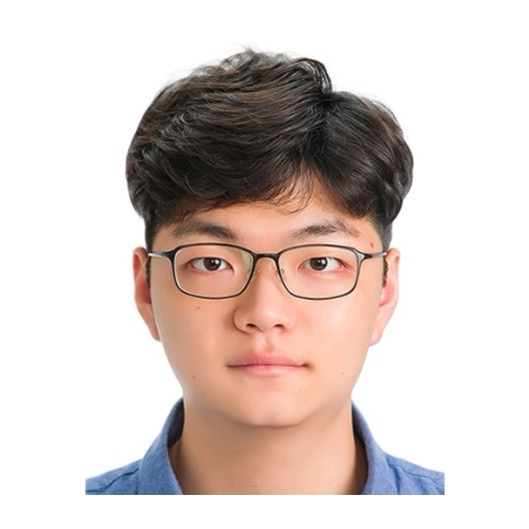
\includegraphics[width = .25\linewidth]{../refs/mugshot.png}}}
  % \vspace{10pt}
    \\ \hline
  \end{tabular}

  \begin{center}
    \begin{tabular}{ p{.2\linewidth}  p{.8\linewidth}}
      {\Large 학력} & \\[10pt]
      \TIME{2018년 3월} &
        {\large 서울대학교 전기정보공학부 학사과정} \newline
        2024년 졸업 예정 \newline
        \textbf{관심 분야}: 딥러닝, 시스템 프로그래밍,
        디지털 시스템 및 하드웨어 디자인 \newline
        \textbf{졸업프로젝트}: CNN 아키텍쳐 디지털 하드웨어 디자인 및 최적화
      % \\[5pt]
    % \TIME{2015년 3월}[2018년 2월] &
    %   {\large Sangmoon High School}
      \\[10pt]
      {\Large 경력} & \\[10pt]
      \TIME{2019년 12월}[2021년 7월] &
        {\large KATUSA, 인사행정병 (311.101)} \newline
        \textbf{미 8군 94군사경찰대대}, 평택, 대한민국
        \begin{itemize}
          \item KATUSA 요원으로 군 의무 복무
        \end{itemize}
      \\[-5pt]
      \TIME{2023년 1월} &
        {\large 서울대학교 연합전공 인공지능반도체공학 학생인턴} \newline
        \textbf{서울대학교}, 서울, 대한민국
        \begin{itemize}
          \item CNN 아키텍쳐와 하드웨어 디자인 최적화 연구
        \end{itemize}
      \\[-5pt]
      \TIME{2023년 3월} &
        {\large 뉴로리얼리티비전 FPGA 엔지니어 인턴} \newline
        동탄, 대한민국
      \\[10pt]
    % {\Large Publications} & \\[10pt]
    % \TIME{<++>} &
    %   <++>
    % \\[20pt]
      {\Large 능력} & \\[10pt]
      \HEAD{공학} & \vspace{-\baselineskip}
        \begin{itemize}
          \item C, C++ and Python 기초 수준
          \item 범용 FPGA의 임베디드 시스템 설계 경험
          \item Verilog 사용 하드웨어 디자인 경험
          \item HTML/CSS 프론트엔드 개발 프로젝트 경험
          \item \LaTeX{} 조판 숙련
        \end{itemize}
        \\[-5pt]
      \HEAD{언어} & \vspace{-\baselineskip}
        \begin{itemize}
          \item 한국어: 모국어 수준
          \item 영어: 자유로운 의사소통 가능
        \end{itemize}
      \\
    \end{tabular}
  \end{center}

\end{document}
